\documentclass{fizykalab}

% Variables
\def\pomvspace{\vspace{0.3em}}

% Ustawienia strony
\usepackage{lipsum}
\usepackage[margin=3cm]{geometry}
\usepackage{graphicx}
\usepackage{enumitem}
\usepackage{siunitx}
\usepackage{amsmath}
\usepackage{cancel}
\usepackage{makecell}
\usepackage{mathtools}
\usepackage{soul}
\setlist{leftmargin=15pt,labelindent=15pt}
\setlist[enumerate]{noitemsep,wide=0pt, leftmargin=*}

% Ustawienia stopki
\usepackage{lastpage}
\usepackage{fancyhdr}
\pagestyle{fancy}
\fancyhf{} % sets both header and footer to nothing
\renewcommand{\headrulewidth}{0pt}
\cfoot{\thepage\ z \pageref{LastPage}}

% Ustawienia do tabelki
\wydzial{IEiT}
\autorjeden{Robert Mesek}
\autordwa{}
\rok{II}
\grupa{8 - L}
\zespol{6}
\temat{Spektrometr optyczny}
\nrcwiczenia{83}
\datawykonania{14.11.2023}
\dataoddaniajeden{}
\zwrotdopoprawy{}
\dataoddaniadwa{}
\datazaliczenia{}

\begin{document}

\maketitle
{\setlength{\parindent}{0pt}
\section*{Ćwiczenie "83": Spektrometr optyczny}
\subsection*{Cel ćwiczenia}
\par
Celem ćwiczenia jest wyznaczenie długości fal widma liniowe par rtęci za pomocą spektrometru z siatką dyfrakcyjną.

\subsection*{Opis ćwiczenia}
\par
Spektrometria jest nauką o powstawaniu i analizie widm spektroskopowych. Zajmuje się ona badaniem widm promieniowania emitowanego lub absorbowanego przez badaną substancję. Na zajęciach zajmujemy się spektrometrią optyczną. Za pomocą pomiaru widma promieniowania możemy dokonać analizy struktury poziomów energetycznych atomów. Istnieje dyskretnych poziomów energetycznych skutkuje występowaniem widma liniowego. Zgodnie z postulatem Bohra, emisja kwantu o danej energii jest wynikiem przejścia elektronu z poziomu o energii wyższej na poziom o energii niższej, gdzie emitowana energia jest wówczas różnicą energii między poziomami i określa się ona wzorem:
\begin{gather*}
	hv = E_j - E_i \ .
	\tag{1}
\end{gather*}
\begin{flalign*}
	\text{gdzie: } \quad \quad h \  & - \ \text{stała Plancka} &  & \\
	v \                             & - \ \text{szybkość fali}  &  & \\
	E_j \                       & - \ \text{j-ty poziom o wyższej energii} &  & \\
	E_i \                       & - \ \text{i-ty poziom o niższej energii} &  & 
\end{flalign*}

Będziemy badać widmo światła widzialnego za pomocą spektrometru optycznego i zawartej w nim siatki dyfrakcyjnej, która pozwoli na rozszczepienie wiązki świetlnej. W wyniku interferencji światła przechodzącego przez siatkę otrzymamy szereg wiązek ugiętych opisanych wzorem:
\begin{gather*}
	\sin{\alpha} = \frac{n \lambda}{d} \ .
	\tag{2}
\end{gather*}
\begin{flalign*}
	\text{gdzie: } \quad \quad \alpha \  & - \ \text{kąt padania wiązki} &  & \\
	d \                             & - \ \text{stała siatki}  &  & \\
	\lambda \                       & - \ \text{długość fali} &  & \\
	n \                       & - \ \text{rząd widma} &  & 
\end{flalign*}

\newpage

\section*{Stanowisko pomiarowe}
\begin{figure}[!ht]
	\centering
	\vspace{0pt}
	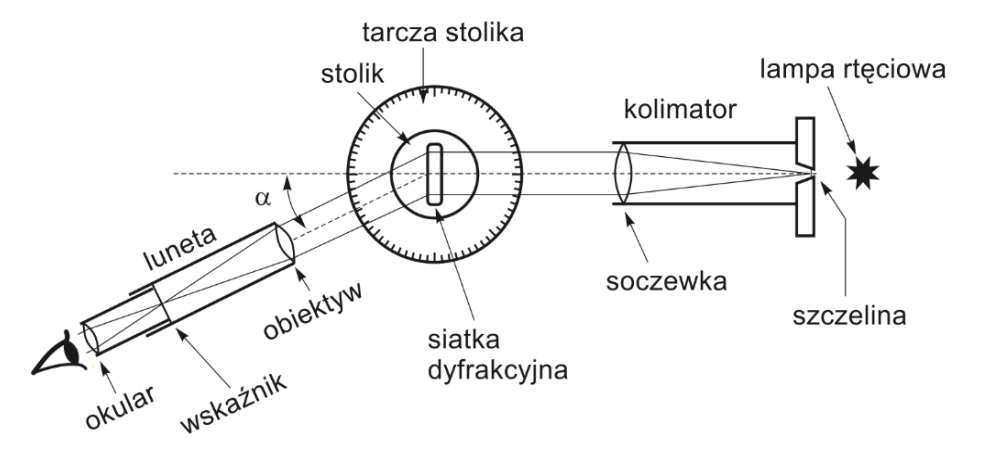
\includegraphics[width=0.9\linewidth]{images/uklad1.png}
	\caption*{Rys. 1 Układ pomiarowy}
\end{figure}



\section*{Przebieg doświadczenia}
\par
Przygotowanie do pomiarów:
\begin{enumerate}
	\item Zapalenie lampy rtęciowej i jej ustawienie.
	
	\item Ustawienie szerokości szczeliny i siatki dyfrakcyjnej.
	
	\item Zaznajomienie się z mechanizmem obrotu lunety oraz regulacja ostrości i obserwacja widma.
\end{enumerate}

Zapisanie wyników:
\begin{enumerate}
	\item Odczytanie wartości kąta dla wiązki nieodchylonej.
	
	\item Znalezienie kolejnych prążków w skutku rozszczepienia światła i odczytanie ich kąta padania.
\end{enumerate}

\newpage

\section*{Wyniki pomiarów}
\par
\begin{table}[H]
	\centering
	\begin{tabular}{|l|}
		\hline
		\rule{0pt}{1em} \textbf{Szczegóły stanowiska pomiarowego} \\ \hline\hline
		\rule{0pt}{1em} Lampa Hg \\ \hline
		\rule{0pt}{1em} Siatka dyfrakcyjna 570/mm \\ \hline
	\end{tabular}
	\caption*{Tabela 1: Dane przyrządów.}
\end{table}

\section*{Oczytane wartości}
\par
Przekreślone wartości zostały uznane za błędy grube. Wskazują na to fakty: prążki te były niewyraźne (znacznie różniące się od pozostałych), wystąpiły tylko z prawej strony (nie symetryczne) oraz po podstawieniu do wzoru nie pokrywają się z wartościami tabelarycznymi.

Najprawdopodobniej były to odbicia wewnętrzne lub refleksy pochodzące z innego źródła światłą niż lampa rtęciowa.
\begin{table}[H]
	\centering
\begin{tabular}{|l|l|l|l|l|l|}
	\hline
	\rule{0pt}{1em} \textbf{Strona} & \textbf{Rząd} & \textbf{Stopnie [°]} & \textbf{Minuty [']} & \textbf{Kolor} & \textbf{Odchylenie [°]} \\ \hline\hline
	\rule{0pt}{1em} Środek & 0 & 0 & 0 & biały & 0 \\ \hline\hline
	\rule{0pt}{1em} Prawa & 1 & 345 & 32 & fioletowy & 14.47 \\ \hline
	\rule{0pt}{1em} Prawa & 1 & 341 & 49 & zielony & 18.18 \\ \hline
	\rule{0pt}{1em} Prawa & 1 & 340 & 45 & pomarańczowy & 19.25 \\ \hline
	\rule{0pt}{1em} \st{Prawa} & \st{2} & \st{334} & \st{56} & \st{fioletowy} & \st{25.07} \\ \hline
	\rule{0pt}{1em} \st{Prawa} & \st{2} & \st{330} & \st{49} & \st{zielony} & \st{29.18} \\ \hline
	\rule{0pt}{1em} Prawa & 2 & 330 & 0 & fioletowy & 30.00 \\ \hline
	\rule{0pt}{1em} \st{Prawa} & \st{2} & \st{329} & \st{35} & \st{pomarańczowy} & \st{30.42} \\ \hline
	\rule{0pt}{1em} Prawa & 2 & 321 & 15 & zielony & 38.75 \\ \hline
	\rule{0pt}{1em} Prawa & 2 & 318 & 30 & pomarańczowy & 41.50 \\ \hline
	\rule{0pt}{1em} Prawa & 2 & 318 & 24 & pomarańczowy & 41.60 \\ \hline\hline
	\rule{0pt}{1em} Lewa & 1 & 14 & 30 & fioletowy & 14.50 \\ \hline
	\rule{0pt}{1em} Lewa & 1 & 18 & 12 & zielony & 18.20 \\ \hline
	\rule{0pt}{1em} Lewa & 1 & 19 & 18 & pomarańczowy & 19.30 \\ \hline
	\rule{0pt}{1em} Lewa & 2 & 29 & 50 & fioletowy & 29.83 \\ \hline
	\rule{0pt}{1em} Lewa & 2 & 38 & 30 & zielony & 38.50 \\ \hline
	\rule{0pt}{1em} Lewa & 2 & 41 & 7 & pomarańczowy & 41.12 \\ \hline
	\rule{0pt}{1em} Lewa & 2 & 41 & 21 & pomarańczowy & 41.35 \\ \hline
\end{tabular}
	\caption*{Tabela 2: Wyniki pomiarów.}
\end{table}

\newpage

\section*{Opracowanie wyników}
\subsection*{Obliczenie długości fali}
\par 
Wzór na długość fali po przekształceniu wzoru (2):
\begin{gather*}
	\lambda  = \frac{d \sin{\alpha}}{n} \ .
	\tag{3} 
\end{gather*}
Źródło wartości tabelarycznych: \verb|lpf.wppt.pwr.edu.pl/opisy/tabela_72_76.pdf|
\begin{table}[H]
	\centering
	\begin{tabular}{|l|l|l|l|l|l|l|}
		\hline
		\textbf{Lp} & \textbf{Rząd} & \makecell{\rule{0pt}{1em} \textbf{Średnie} \\ \textbf{odchylenie [°]}} & \textbf{Kolor} & \makecell{\textbf{Długość} \\ \textbf{fali [nm]}} & \makecell{\textbf{Przewidywana} \\  \textbf{długość fali [nm]}} & \makecell{\textbf{Różnica} \\ \textbf{[nm]}} \\ \hline\hline
		1 & 1 & 14.48 & fioletowy & 438.67 & 434.80 & 3.87 \\ \hline
		2 & 1 & 18.19 & zielony & 547.59 & 546.07 & 1.52 \\ \hline
		3 & 1 & 19.28 & pomarańczowy & 579.00 & 578.02 & 0.98 \\ \hline\hline
		4 & 2 & 29.92 & fioletowy & 437.39 & 434.80 & 2.59 \\ \hline
		5 & 2 & 38.63 & zielony & 547.44 & 546.07 & 1.37 \\ \hline
		6 & 2 & 41.31 & pomarańczowy & 578.92 & 576.96 & 1.96 \\ \hline
		7 & 2 & 41.48 & pomarańczowy & 580.83 & 579.07 & 1.76 \\ \hline
	\end{tabular}
	\caption*{Tabela 3: Porównanie z wartościami tabelarycznymi.}
\end{table}


\subsection*{Niepewności pomiarowe}
\paragraph*{Zgodnie ze skryptem: }
Określenie błędu pomiaru $\Delta \lambda$ jest trudne, gdyż o dokładności pomiaru decyduje nie
precyzja odczytu kąta (która jest bardzo duża), lecz błąd systematyczny wynikający
z niedoskonałego wyjustowania przyrządu. Za szacunkową wartość błędu można przyjąć
średnią różnicę wartości $\lambda$ uzyskanych z widm 1 i 2 rzędu:
\begin{gather*}
	u(\lambda) = 0.77 \ \text{[nm]}
\end{gather*}

\subsection*{Przejścia optyczne w atomie Hg}
\par
Przekształcając wzór (1):
\begin{gather*}
	h\frac{c}{\lambda} = \Delta E \ .
	\tag{4}
\end{gather*}
\begin{flalign*}
	\text{gdzie: } \quad \quad h \  & - \ \text{stała Plancka} &  & \\
	c \                             & - \ \text{prędkość światła}  &  & \\
	\lambda \                       & - \ \text{długość fali} &  & \\
	\Delta E \                       & - \ \text{emitowana energia podczas przejścia} & & 
\end{flalign*}

\begin{table}[H]
	\centering
	\begin{tabular}{|l|l|l|l|l|}
		\hline
		\rule{0pt}{1em} \textbf{Lp} & \textbf{Długość fali [nm]} & \textbf{$\boldsymbol{\Delta E}$ [eV]} & \textbf{Przejście} \\ \hline\hline
		\rule{0pt}{1em}1 & 434.80 & 2.827 & $7_3 S_1 \rightarrow 6^3 P_1$ \\ \hline
		\rule{0pt}{1em}2 & 546.07 & 2.264 & $7_3 S_1 \rightarrow 6^3 P_2$ \\ \hline
		\rule{0pt}{1em}3 & 578.02 & 2.142 & $6^1 D_2 \rightarrow 6^1 P_1$ \\ \hline
	\end{tabular}
	\caption*{Tabela 4: Dopasowanie przejścia optycznego}
\end{table}

\newpage

\section*{Wnioski}
\par
Otrzymane wyniki są zgodne z przewidywanymi oraz wszystkie otrzymane wartości różnią się od wartości tabelarycznych o <1\%.

W doświadczeniu wystąpiły błędy grube związane z refleksami, jednak ich charakterystyka pozwoliła je sklasyfikować i odrzucić.

Dla 1 rzędu otrzymano tylko jeden prążek pomarańczowy (dla 2 rzędu otrzymano dwa). Jest to najprawdopodobniej spowodowane faktem, że odległość miedzy nimi jest bardzo małą, dlatego możemy przyjąć, że ta wartość jest w przybliżeniu średnią dla obu prążków.

Wyznaczenie niepewności pomiarowych w tym przypadku jest nie oczywiste, dlatego wykorzystano radę zawartą w skrypcie odnośnie tego doświadczenia.

\end{document}
